\documentclass[11pt,a4paper]{article}

\usepackage[margin=1in]{geometry}
\usepackage[T1]{fontenc}
\usepackage{lmodern}
\usepackage{amsmath,amssymb}
\usepackage{booktabs}
\usepackage{graphicx}
\usepackage{hyperref}
\usepackage{microtype}

\graphicspath{{figures/}}
\hypersetup{
  colorlinks=true,
  linkcolor=blue,
  citecolor=blue,
  urlcolor=blue
}

\title{Corrected Noninteracting Reproduction Report for the Nonsymmorphic DTC Model}
\author{Python/CUDA reproduction notes}
\date{\today}

\begin{document}
\maketitle

\begin{abstract}
This report documents the corrected noninteracting reproduction stage for the two-level model in Hu, Fu, Li, and Shen, \emph{Physical Review Research} \textbf{5}, L032024 (2023). The calculation now compares both the refined special parameter near \(\alpha_{13}\) and the detuned parameter \(\alpha=81.60\). It also replaces integer-period-only projection sampling with fractional-period sampling at \(0,T/4,T/2,3T/4\).
\end{abstract}

\section{Scope}

The target is the noninteracting two-level Hamiltonian, not the interacting spin-chain lifetime analysis. The implemented workflow generates the time trace, Fourier spectrum, solver-comparison data, fractional-period projection data, validation diagnostics, and figures under \path{reproduction_noninteracting/}. A separate LaTeX supplement, \path{numerical_methods_supplement.tex}, gives the detailed theory of the fourth-order Magnus and RK4 methods.

\section{Model and Units}

The reproduced Hamiltonian is
\begin{equation}
H_0(t)
= \frac{1}{2}\Omega\sin(t)\sigma_x
 + \Omega\sin^2\left(\frac{t}{2}\right)\sigma_y,
\label{eq:h0}
\end{equation}
with \(\hbar=1\) and drive angular frequency \(\omega=1\). Hence
\begin{equation}
T=2\pi,\qquad \alpha=8\Omega,\qquad \Omega=\alpha/8.
\end{equation}
The initial state is
\begin{equation}
|+x\rangle = \frac{1}{\sqrt{2}}\begin{pmatrix}1\\1\end{pmatrix}.
\end{equation}

The main observable is
\begin{equation}
\langle \sigma_x(t)\rangle
= \frac{\langle\psi(t)|\sigma_x|\psi(t)\rangle}
{\langle\psi(t)|\psi(t)\rangle}.
\end{equation}
For this initial state, the \(x\)-spin autocorrelation
\begin{equation}
C_x(t)=\langle +x|U^\dagger(t)\sigma_xU(t)\sigma_x|+x\rangle
\end{equation}
equals \(\langle\sigma_x(t)\rangle\), because \(\sigma_x|+x\rangle=|+x\rangle\). The plotted trace therefore also serves as the requested single-spin \(x\)-autocorrelation for this initial condition.

\section{Numerical Methods}

The main script is \texttt{reproduce\_noninteracting.py}. It uses simple functions with explicit constants near the top of the file.

\subsection{Fourth-Order Magnus Method}

The primary propagator is a fourth-order Magnus method using two Gauss--Legendre nodes. With
\begin{equation}
A(t)=-iH(t),
\end{equation}
the step generator is
\begin{equation}
\Omega_M
= \frac{\Delta t}{2}(A_1+A_2)
 - \frac{\sqrt{3}\Delta t^2}{12}[A_1,A_2],
\end{equation}
and the state update is
\begin{equation}
|\psi(t+\Delta t)\rangle=\exp(\Omega_M)|\psi(t)\rangle.
\end{equation}
Since \(\Omega_M\) is anti-Hermitian for a Hermitian Hamiltonian, this method is unitary up to floating-point error.

\subsection{Runge--Kutta Comparison}

The comparison solver is standard fourth-order Runge--Kutta (RK4) applied directly to the Schrodinger equation. RK4 is fourth-order accurate but is not exactly unitary, so the report tracks norm drift. In the validation run, RK4 uses four substeps per plotted Magnus step, giving an effective RK4 resolution of 320 steps per drive period.

The detailed derivation and implementation rationale for both methods are given in the accompanying numerical-methods supplement.

\section{Parameters}

The paper gives the table value \(\alpha_{13}=80.07\). A high-accuracy SciPy period-evolution minimization refines the nearby zero of the one-period return probability to
\begin{equation}
\alpha_{13}=80.04624211689759.
\end{equation}
The return probability at this refined point is \(3.57\times10^{-18}\). The corrected reproduction uses both this refined value and the detuned noninteracting value
\begin{equation}
\alpha=81.60.
\end{equation}

\section{Validation Diagnostics}

The latest validation run used the local RTX 4090 CUDA device. Table~\ref{tab:diagnostics} summarizes the diagnostics saved in \texttt{data/diagnostics.json}.

\begin{table}[h]
\centering
\caption{Latest noninteracting validation diagnostics.}
\label{tab:diagnostics}
\begin{tabular}{lcc}
\toprule
Quantity & Refined \(\alpha_{13}\) & Detuned \(\alpha=81.60\) \\
\midrule
Parameter value & 80.04624211689759 & 81.60 \\
Magnus4 maximum norm drift & \(4.02\times10^{-5}\) & \(3.92\times10^{-5}\) \\
RK4 maximum norm drift & \(1.59\times10^{-3}\) & \(1.79\times10^{-3}\) \\
Maximum \(\langle\sigma_x\rangle\) solver difference & \(8.35\times10^{-3}\) & \(6.50\times10^{-3}\) \\
Dominant normalized spectrum frequency & 0.4998 & 0.5498 \\
\bottomrule
\end{tabular}
\end{table}

The common settings were CUDA on an NVIDIA GeForce RTX 4090, 40 plotted periods, 80 Magnus steps per period, and 320 effective RK4 steps per period. Fractional projections were sampled at \(0,T/4,T/2,3T/4\) within every period for 60 periods.

\section{Generated Figures}

Figure~\ref{fig:param-comparison} compares the noninteracting dynamics for the refined \(\alpha_{13}\) and the detuned value \(\alpha=81.60\). The refined parameter locks the dominant response close to \(\tilde{\omega}/\omega=1/2\). The detuned value shows additional Fourier features, reproducing the qualitative behavior emphasized in the paper's Fig.~4(a): without interactions, detuning from \(\alpha_n\) allows fast off-diagonal oscillations to dominate the observable.

\begin{figure}[p]
\centering
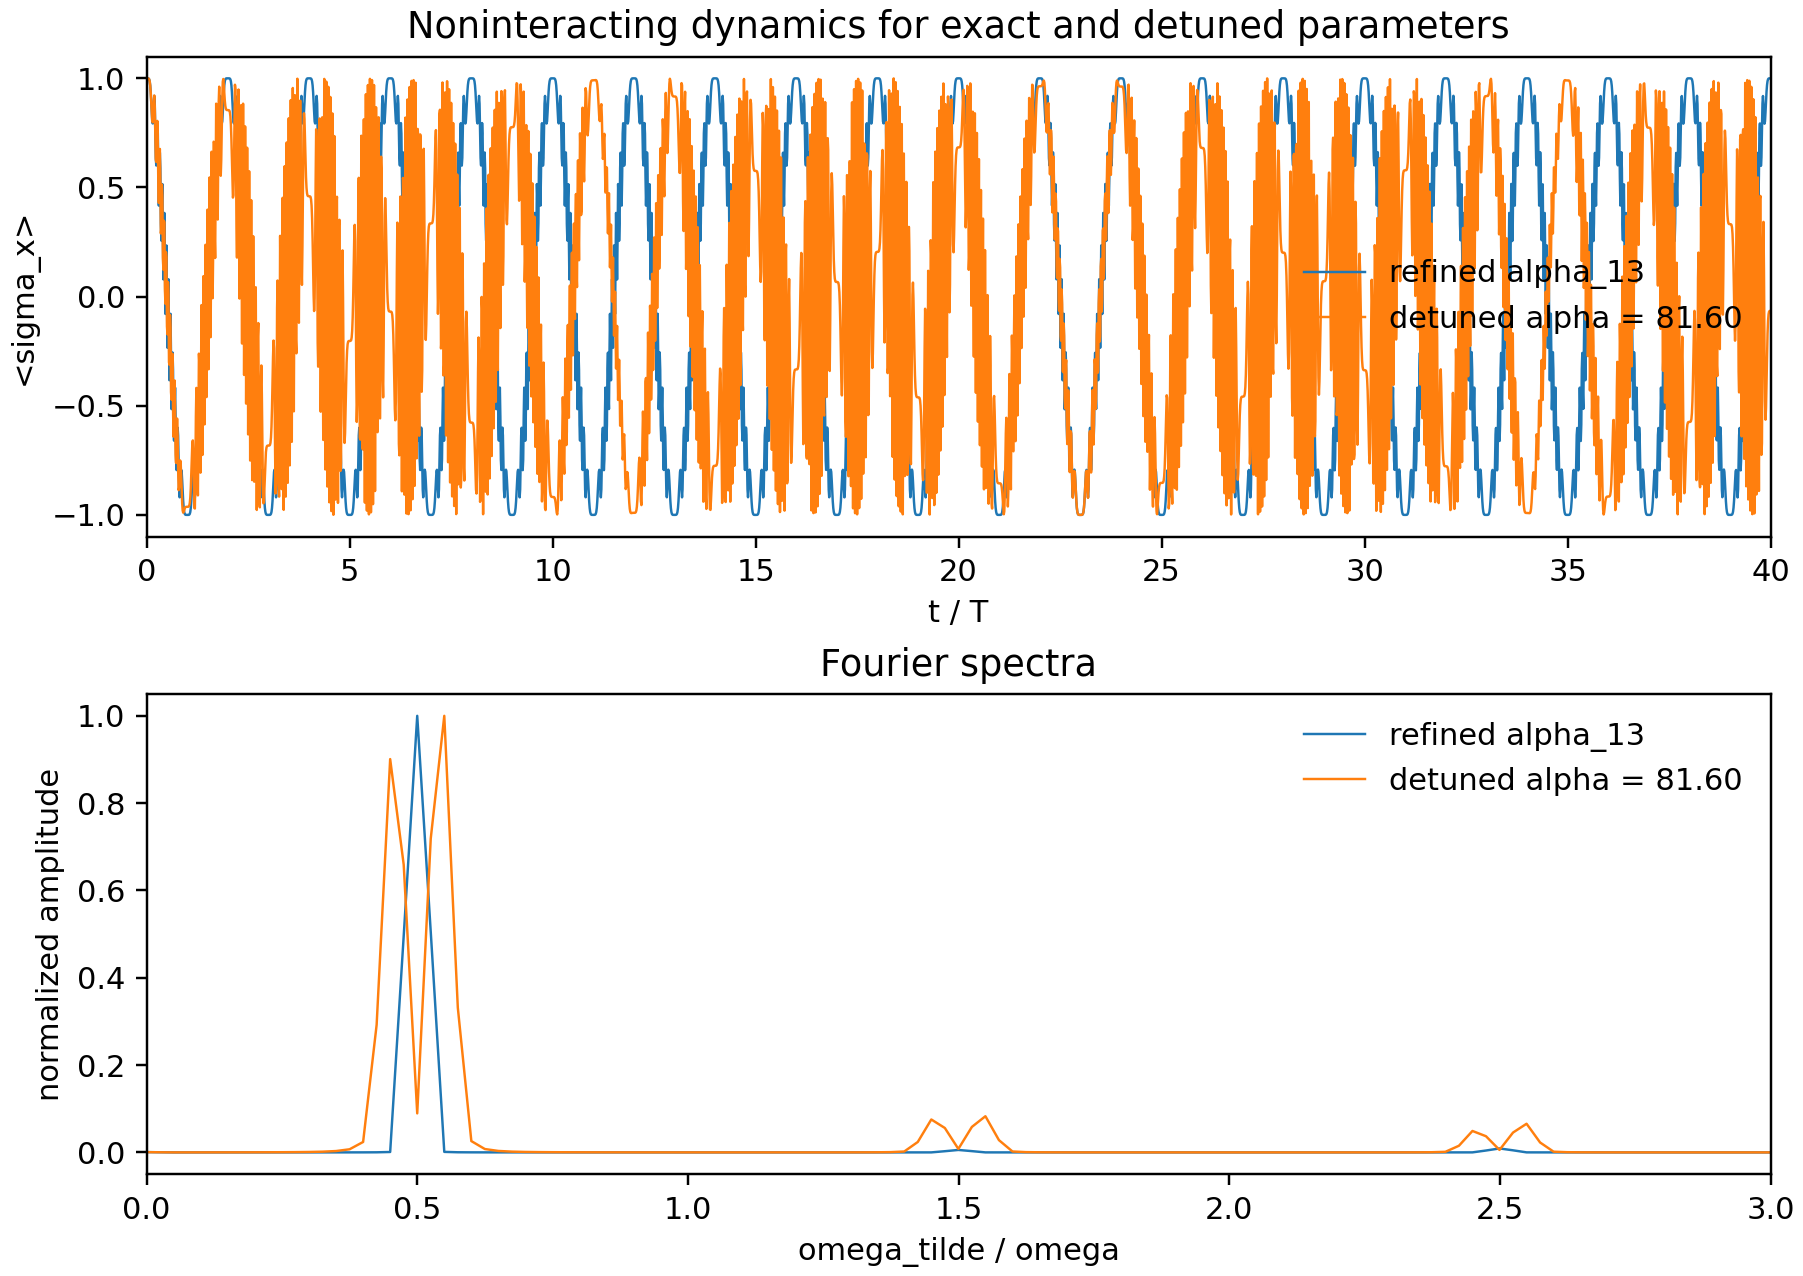
\includegraphics[width=0.95\linewidth]{sigma_x_parameter_comparison.png}
\caption{Noninteracting \(\langle\sigma_x(t)\rangle\) and Fourier spectra for the refined \(\alpha_{13}\) and the detuned value \(\alpha=81.60\).}
\label{fig:param-comparison}
\end{figure}

Figures~\ref{fig:solver-alpha13} and \ref{fig:solver-detuned} compare the Magnus4 and RK4 traces for the two parameters. The two observables agree closely at the chosen resolution, while the norm-drift panels show the expected advantage of the unitary Magnus update.

\begin{figure}[p]
\centering
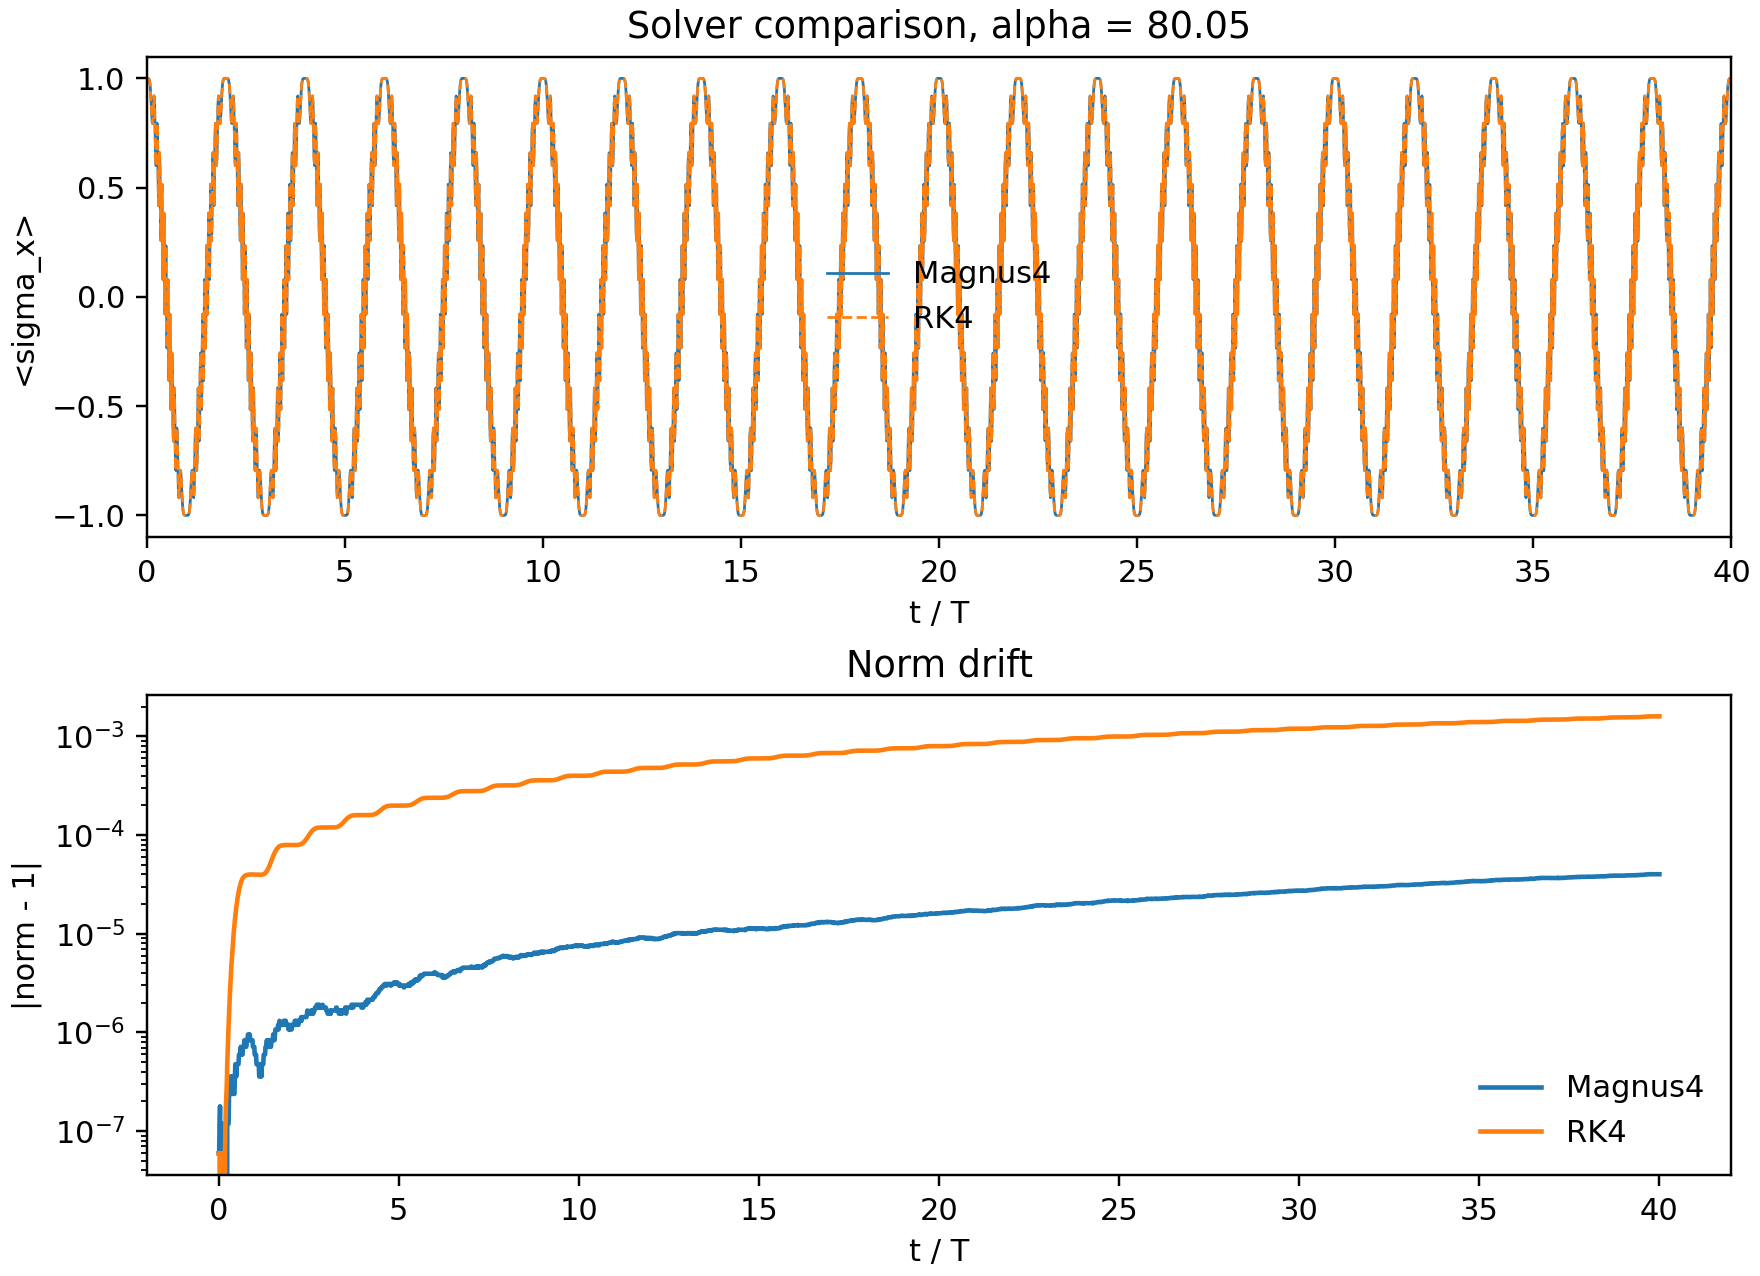
\includegraphics[width=0.95\linewidth]{magnus_rk4_comparison_alpha_13.png}
\caption{Solver comparison for the refined \(\alpha_{13}\). RK4 uses four substeps per plotted Magnus step.}
\label{fig:solver-alpha13}
\end{figure}

\begin{figure}[p]
\centering
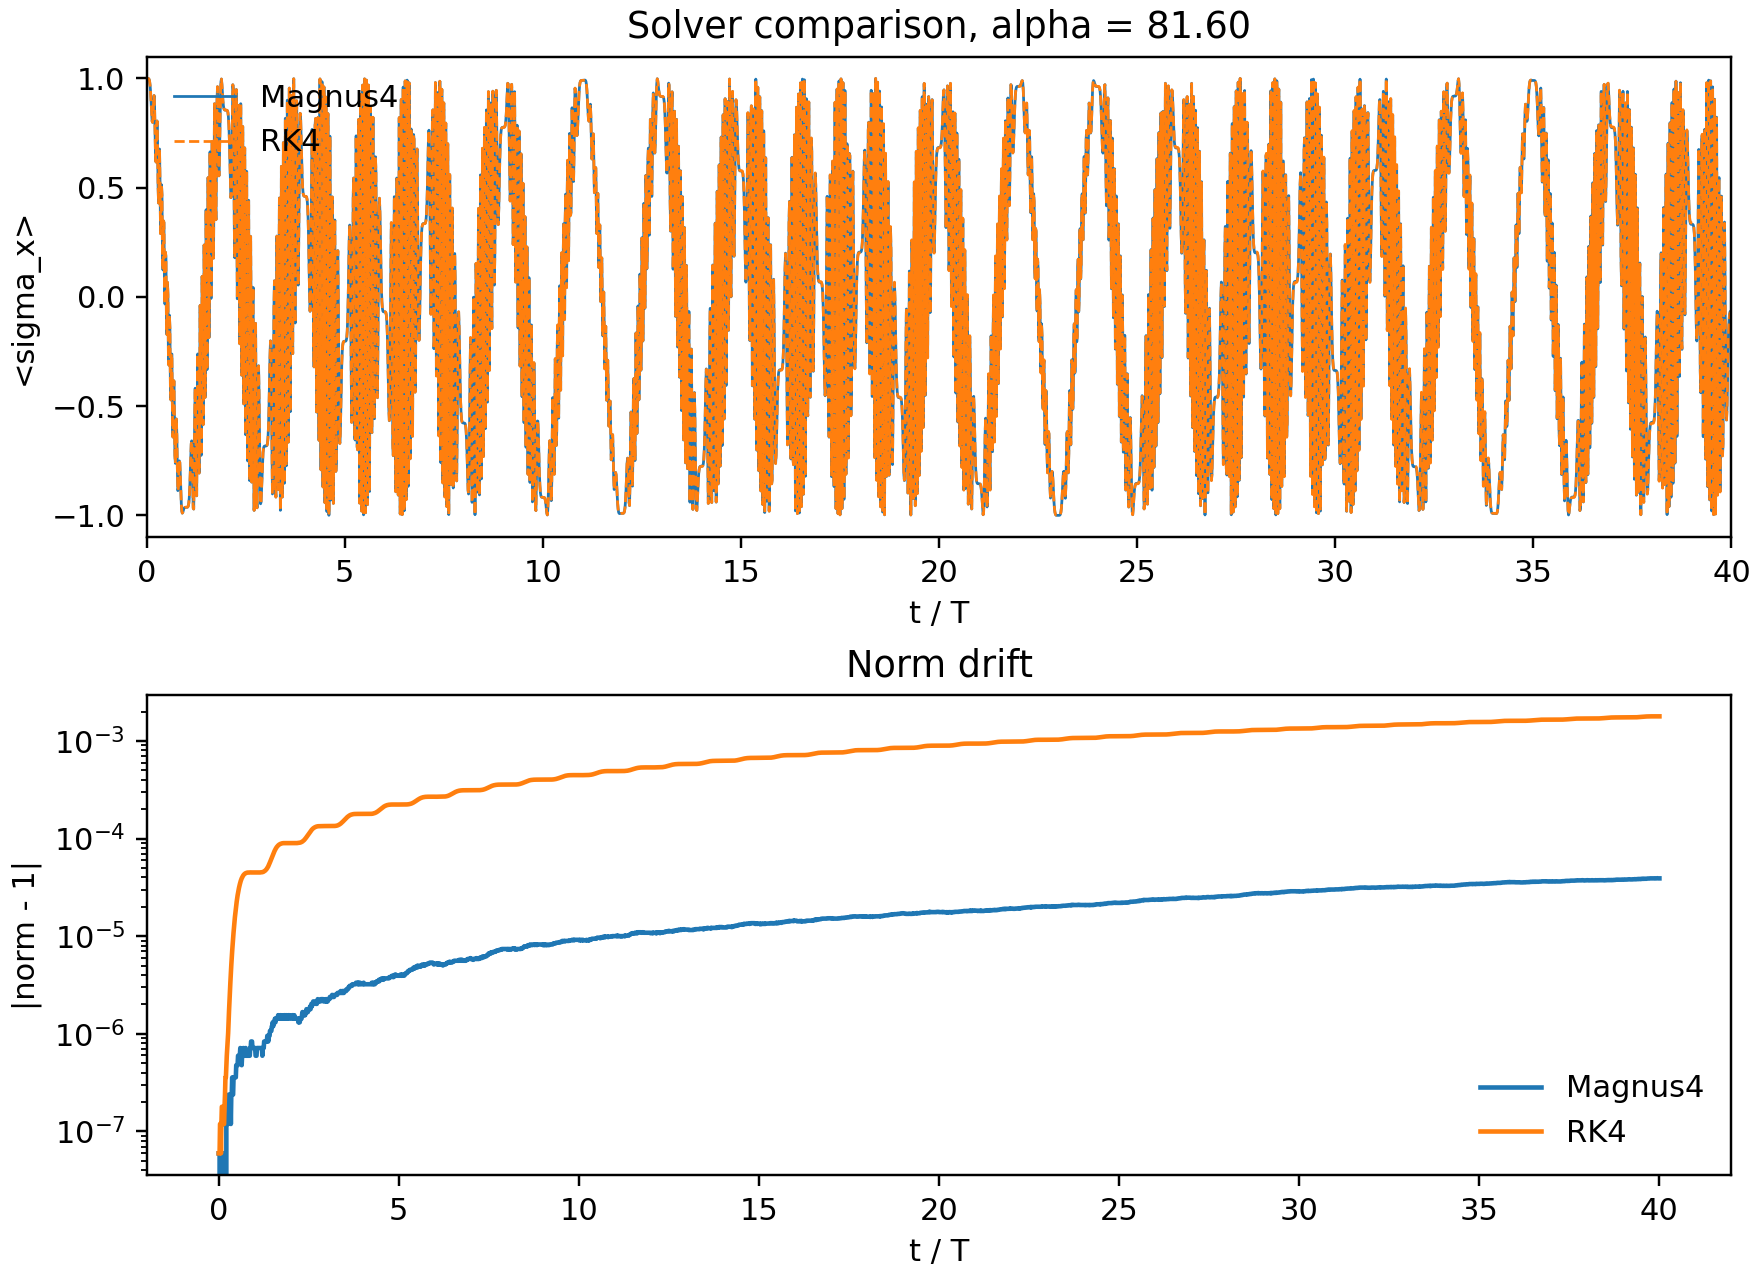
\includegraphics[width=0.95\linewidth]{magnus_rk4_comparison_alpha_81p60.png}
\caption{Solver comparison for the detuned value \(\alpha=81.60\). RK4 uses four substeps per plotted Magnus step.}
\label{fig:solver-detuned}
\end{figure}

Figure~\ref{fig:fractional} shows fractional-period projections sampled at \(0,T/4,T/2,3T/4\) within every period. This implements the correction that the projection analysis should not be restricted to integer periods. For the refined \(\alpha_{13}\), the sampled points form a small number of fixed-point clusters. For the detuned value, the points spread along the quarter circle.

\begin{figure}[p]
\centering
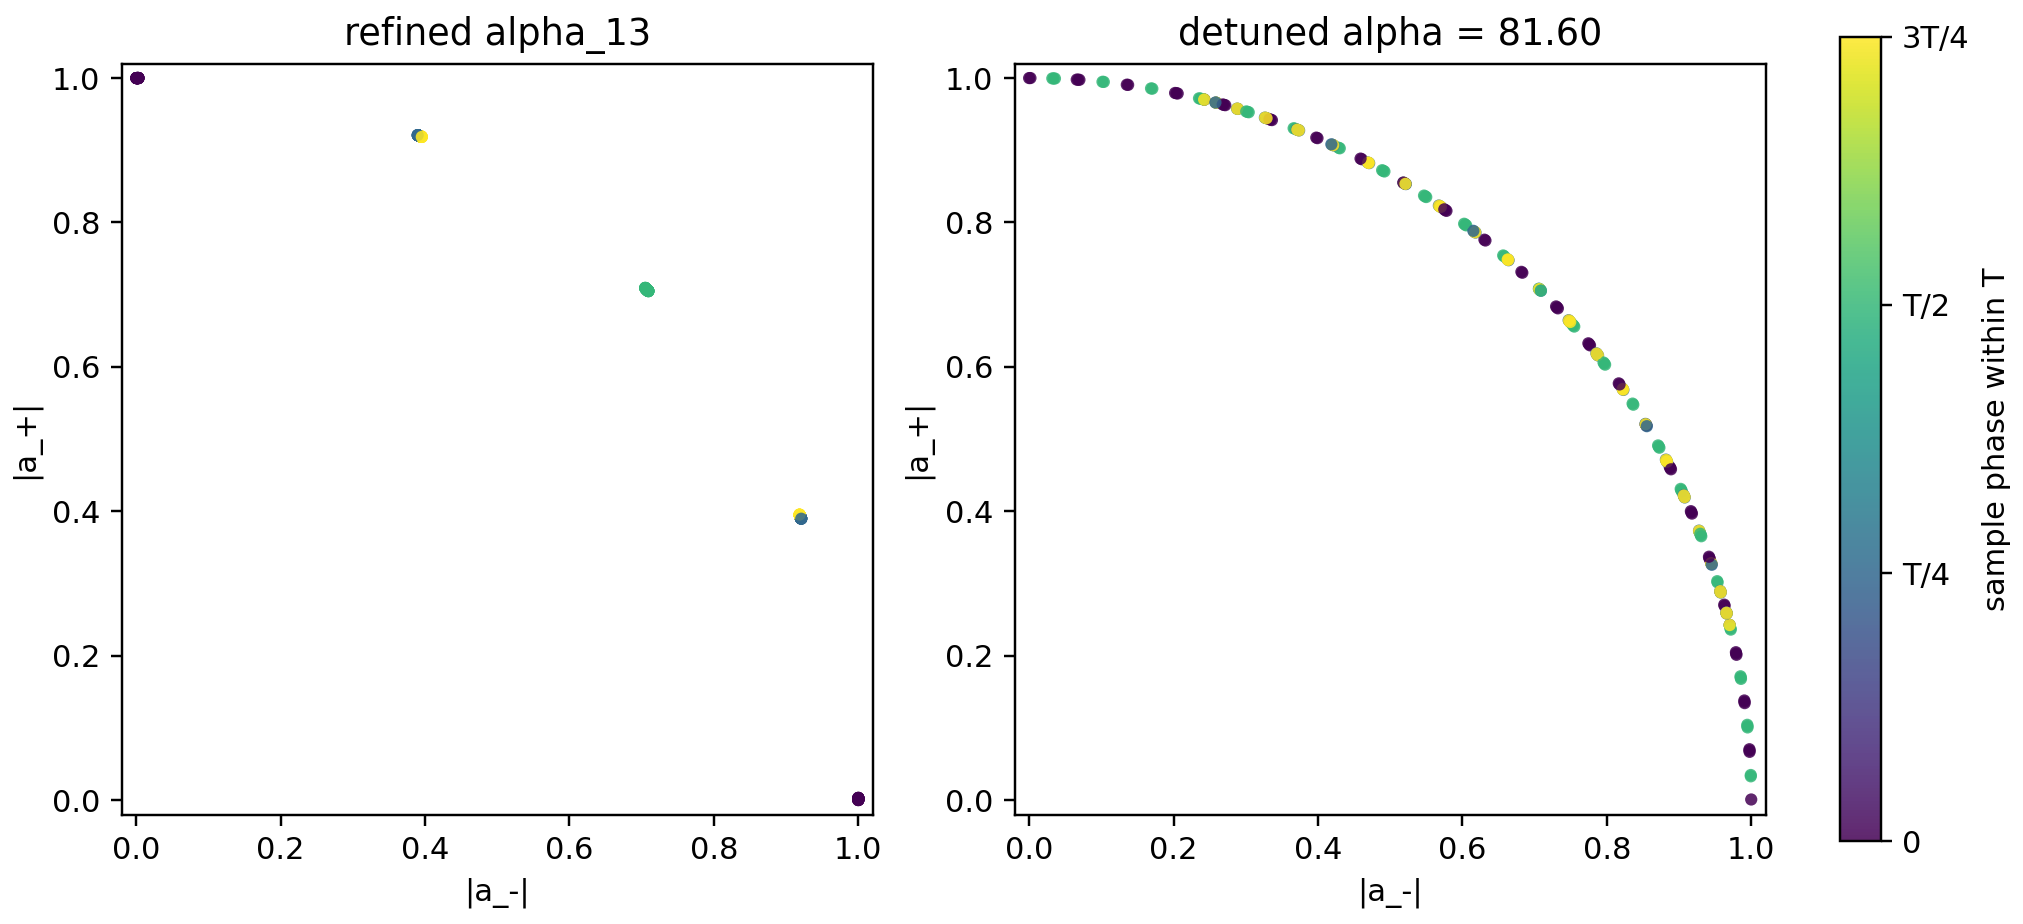
\includegraphics[width=0.95\linewidth]{fractional_projections_parameter_comparison.png}
\caption{Fractional-period projections for the refined \(\alpha_{13}\) and the detuned value \(\alpha=81.60\). Colors indicate the sample phase \(0,T/4,T/2,3T/4\) within each drive period.}
\label{fig:fractional}
\end{figure}

\section{Generated Data}

The reproduction run generates the following files:
\begin{itemize}
  \item \texttt{data/sigma\_x\_alpha\_13.csv};
  \item \texttt{data/sigma\_x\_alpha\_81p60.csv};
  \item \texttt{data/spectrum\_alpha\_13.csv};
  \item \texttt{data/spectrum\_alpha\_81p60.csv};
  \item \texttt{data/fractional\_projections\_alpha\_13.csv};
  \item \texttt{data/fractional\_projections\_alpha\_81p60.csv};
  \item \texttt{data/stroboscopic\_alpha\_13.csv};
  \item \texttt{data/diagnostics.json};
  \item \texttt{figures/sigma\_x\_parameter\_comparison.png};
  \item \texttt{figures/sigma\_x\_alpha\_13.png};
  \item \texttt{figures/sigma\_x\_alpha\_81p60.png};
  \item \texttt{figures/magnus\_rk4\_comparison\_alpha\_13.png};
  \item \texttt{figures/magnus\_rk4\_comparison\_alpha\_81p60.png};
  \item \texttt{figures/fractional\_projections\_parameter\_comparison.png};
  \item \texttt{figures/fractional\_projections\_alpha\_13.png};
  \item \texttt{figures/fractional\_projections\_alpha\_81p60.png};
  \item \texttt{figures/stroboscopic\_alpha\_13.png};
  \item \texttt{numerical\_methods\_supplement.tex};
  \item \texttt{numerical\_methods\_supplement.pdf}.
\end{itemize}

\section{Limitations}

The code does not directly evaluate confluent Heun functions. Instead, it refines \(\alpha_{13}\) using high-accuracy period evolution under the Hamiltonian itself. This is adequate for this stage because the numerical dynamics are generated from Eq.~\eqref{eq:h0}. The fractional-period projection is performed in the fixed \(\phi_\pm(0)\), or \(\pm x\), basis. The interacting many-body Hamiltonian and finite-size prethermal lifetime analysis remain future work.

\section{Conclusion}

The corrected noninteracting reproduction verifies the central single-spin mechanism for both the refined special parameter and a nearby detuned parameter. At the refined \(\alpha_{13}\), the dominant spectral response is locked near one half of the drive frequency and fractional-period projections form a small set of fixed points. At \(\alpha=81.60\), the observable develops additional oscillatory structure and the fractional projections spread, matching the qualitative role of the noninteracting comparison in the paper. The fourth-order Magnus solver provides a unitary baseline, while RK4 gives an independent fourth-order comparison.

\end{document}
